\documentclass[11pt]{beamer}
% \documentclass[11pt,handout]{beamer}
\usepackage[T1]{fontenc}
\usepackage[utf8]{inputenc}
\usepackage{float, afterpage, rotating, graphicx}
\usepackage{epstopdf}
\usepackage{longtable, booktabs, tabularx}
\usepackage{fancyvrb, moreverb, relsize}
\usepackage{eurosym, calc}
\usepackage{amsmath, amssymb, amsfonts, amsthm, bm} 


\usepackage[
    natbib=true,
    bibencoding=inputenc,
    bibstyle=authoryear-ibid,
    citestyle=authoryear-comp,
    maxcitenames=3,
    maxbibnames=10,
    useprefix=false,
    sortcites=true,
    backend=biber
]{biblatex}
\AtBeginDocument{\toggletrue{blx@useprefix}}
\AtBeginBibliography{\togglefalse{blx@useprefix}}
\setlength{\bibitemsep}{1.5ex}
\addbibresource{refs.bib}



\hypersetup{colorlinks=true, linkcolor=black, anchorcolor=black, citecolor=black, filecolor=black, menucolor=black, runcolor=black, urlcolor=black}

\setbeamertemplate{footline}[frame number]
\setbeamertemplate{navigation symbols}{}
\setbeamertemplate{frametitle}{\centering\vspace{1ex}\insertframetitle\par}


\begin{document}

\title{Skills and Wages}

\author[Poooja Bansal]
{
{\bf Poooja Bansal}\\
{\small University of Bonn}\\[1ex]
}


\begin{frame}
    \titlepage
    \note{~}
\end{frame}


\begin{frame}[t]
    \frametitle{Introduction}
Many empirical studies have recognized the importance of
non-cognitive skills along with the cognitive skills and we build on this
by :

	\begin{itemize}

		\item first examining whether cognitive and non-cognitive skills explain
difference in hourly wages after controlling for experience and
schooling

		\item Secondly we analyze how these skills affect the wage profiles of
individuals across different occupational levels, since the
requirements for these skills vary with different occupations.
 	\end{itemize}
    	\note{~}
\end{frame}

\begin{frame}[t]

People typically embody both type of skills: Cognitive skills driving their reasoning
and thinking; and non-cognitive skills incorporating their personality traits.
 	\begin{itemize}


		\item There are numerous studies that have established measurements for cognitive
abilities, for instance AFQT scores, GAT scores test and IQ performance tests by
DIW,

		\item Many economists have produced large body of evidence that employers in labor
market have now recognized the relationship between non-cognitive skills and
productivity. This recognition have led to the evolution of measures like
Rosenberg Self esteem scale and Rotter Locus of control, the Big Five Factor
Model.
 	\end{itemize}
\end{frame}

\begin{frame}[t]
	\begin{itemize}
		\item But to what extent is occupation useful to understand how education
and skills are related with wages?

		\item With the rapidly changing trends in the global labor market,
employers today want their employees to possess a certain degree of
qualification, in terms of skills, education and experience, due to the
non-pecuniary characteristics of different jobs.

		\item And in this highly competitive market, employees are keen to develop
their qualifications to suit the market needs. Hence we see how these
qualifications change in the occupational hierarchy.
 	\end{itemize}
\end{frame}

\begin{frame}[t]
    \frametitle{Literature}
    \begin{itemize}
   	 \item There have been numerous studies which investigated the effect of
cognitive skills and personality traits on wages.
  	 \item \citet{heineck} confirms that employers highly value
individuals’ skills. \citet{farkas} also confirm that
employers assess cognitive and non-cognitive skills for hiring,
promotion and wage setting policies.
      
     \end{itemize}
    \note{~}
\end{frame}


\begin{frame}[t]
      On one hand, some studies suggested substantial returns to
cognitive skills :
	 \begin{itemize}
		\item \citet{heineck} have established a positive
relationship between cognitive skills and labor market outcomes,
suggesting that abilities are correlated to the wages in a significantly
positive way for German workers.

		\item citet{levy} also recognized the importance of
cognitive skills in wage determination.
	\end{itemize}
	
While on the other hand, many research works found that cognitive
ability has a very little or no effect on earnings:
	\begin{itemize}
\item \citet{heckman} and \citet{zax} reported
that the effect of cognitive skills is much smaller than what has been
asserted by previous analyses and is rather a poor estimator of
earnings.
	\end{itemize}
         \note{~}
\end{frame}


\begin{frame}[t]
    \begin{itemize}
     	\item \citet[Osborn] explained how some personality traits
matter for employers because they facilitate the production of effort
at work and affect labour productivity.
	\item \citet{Urzua} suggested that non- cognitive skill is
an equally strong determinant, if not more, as cognitive skill.
	\item \citet{Gintis} and \citet{Edwards} in their work showed
that skills such as dependability and persistence are highly valued by
employers.
     \end{itemize}
     \note{~}
\end{frame}


\begin{frame}[t]
	\frametitle{Expectations}
	\begin{itemize}
		\item We expect cognitive skills to have either positive or no association
with the earnings.
		\item With respect to the personality traits used, we expect no significant
relation between Extraversion and wages, a positive relationship for
Openness and conscientiousness and negative for Neuroticism and
Agreeableness.

		\item For occupations, we expect cognitive skills to be either positively or
not related to the occupational categories. For personality traits, we
expect more heterogeneous results for each category of occupation,
depending on their work task and roles.
	 \end{itemize}
 	\note{~}
\end{frame}

\begin{frame}[t]
	\frametitle{Data}
         \begin{itemize}

 
		 \item SOEP is a wide-ranging representative micro-database providing
comprehensive socio- economic information on private households in
Germany.

		\item The panel was first started in 1984 and data for about 12,200
randomly selected respondents, in West Germany, was collected.

		\item We use two recent waves which include data on cognitive skills
(2005), two short verbal and performance tests, and personality traits
(2006), items pertaining to the Big Five Factor model.

		\item We retrieved the data for occupation and education from the
personal questionnaire of 2005.
	\end{itemize}
	\note{~}
\end{frame}

\begin{frame}[t]
	\frametitle{Measures of Cognitive Skills}
	 \begin{itemize}
	 	\item The organization conducted two short tests to evaluate cognitive
skills in year 2006. These were: A Word Fluency Test and Symbol
Correspondence Test.

		\item For the Word Fluency test, respondents were asked to name as many
animals as possible in 90 seconds

		\item For the Symbol Recognition Test respondents had to match as many
number and symbols as possible in 90 seconds using the
correspondence list provided to them.
	\end{itemize}
\end{frame}

\begin{frame}[t]
	\frametitle{Measures of Non-Cognitive Skills}
	We have used the Big Five Factor model to measure the
non-cognitive skills (OCEAN).

	 \begin{itemize}
	 	
		\item Openness

		\item Conscientiousness

		\item Extraversion

		\item Agreeableness

		\item Neuroticism
	 \end{itemize}
\end{frame}

\begin{frame}[t]
	\frametitle{Determination of Hourly Wages}
	 \begin{itemize}
	 	\item SOEP provides data on monthly income from primary employment
and actual weekly working hours including overtime.

		\item We calculate the hourly wages by dividing the monthly income with
the product of weekly hours and the estimated factor of 4.3 for the
number of weeks.

		\item For individuals reporting zero wages, a small value of 0.0001 was
assigned before it was transformed to a logarithmic scale.
	\end{itemize}
\end{frame}

\begin{table}
	\caption{SOEP questions and personality traits used in the analysis }
	\begin{tabular}{l c |  c }
 		Variable label    & Personality traits \\
 		I see myself as someone who ...&\\
 		\hline
 		is original, comes up with new ideas  &Openness \ \\
 		values artistic experiences&Openness \\
 		has an active imagination&Openness\\
 		
 		does a thorough job&   Conscientiousness \\
 		does things effectively and efficiently &Conscientiousness \\
 		tends to be lazy (reversed) &Conscientiousness   \\
		
 		is communicative, talkative&   Extraversion \\
	 	is outgoing, sociable& Extraversion \\
 		is reserved (reversed)& Extraversion \\
 		
 		is sometimes somewhat rude to others (reversed)&Agreeableness\\
 		has a forgiving nature&Agreeableness \\
 		is considerate and kind to others&Agreeableness \\
 	
 		worries a lot&Neuroticism\\
 		gets nervous easily&Neuroticism \\
 		is relaxed, handles stress well (reversed)& Neuroticism\\
 		
	\end{tabular}
\end{table}

\begin{table}
	\caption{Erikson-Goldthorpe Class Categories }
	\begin{tabular}{| c | c }
 	Category&Occupation   \\
 	\hline
	 I &Higher-grade professionals, administrators, and officials\\

 	II &Lower-grade professionals, administrators, and officials \\

	 IIIa &Routine non-manual employees(administration)\\

 	IIIb& Routine non-manual employees (sales and services) \\
 
	IVc &Small proprietors with employee \\
 
	 IVb &Small proprietors without employee  \\

	IVc& Farmers and smallholders, workers in primary production\\

	V& Lower-grade technicians,supervisors of manual workers\\

	VI& Skilled manual workers\\

	VIIa&Semi-skilled and unskilled manual workers  \\

	VIIb&Semi-skilled and unskilled manual workers \\

	\end{tabular}
\end{table}

\begin{figure}
    \caption{Frequency Distribution of Occupation}
    
    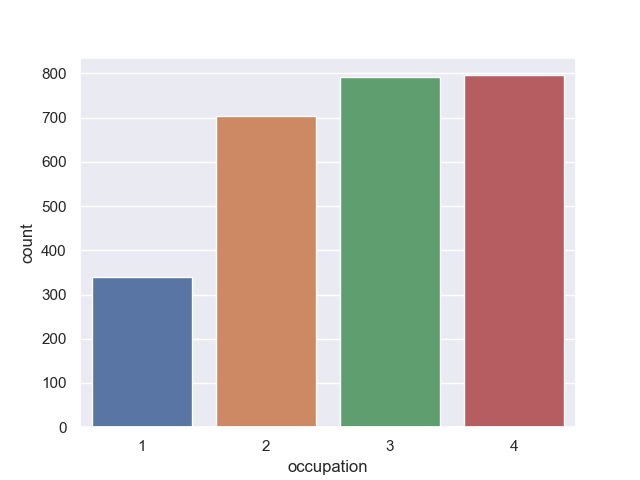
\includegraphics[width=\textwidth]{../../out/figures/occupation_count}

\end{figure}

\begin{figure}
    \caption{Correlation heatmap}
    
    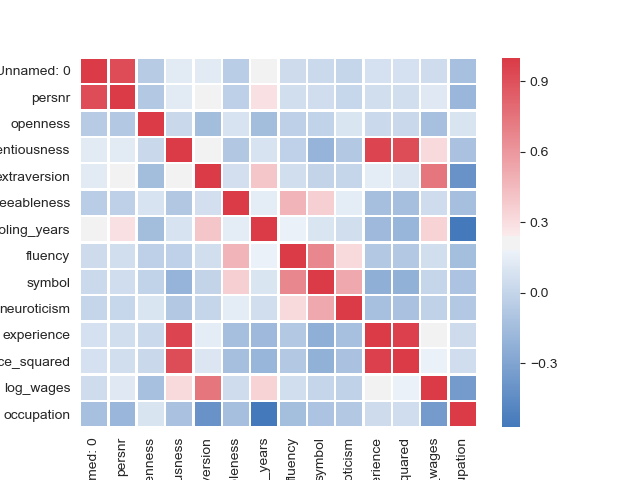
\includegraphics[width=\textwidth]{../../out/figures/heatmap}

\end{figure}

\begin{figure}
    \caption{Density plot for all the variables}
    
    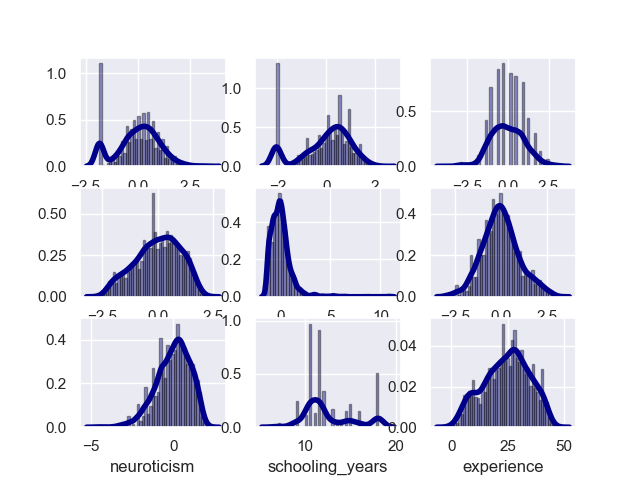
\includegraphics[width=\textwidth]{../../out/figures/distplot}

\end{figure}

\begin{frame}[t]
	\frametitle{Analytical Sample}
	 \begin{itemize}
	 	\item To address the research question posted in the study, the analytical
sample is limited to individuals between age 20 and 60 who were in
full time employment, in order to include only those who most likely
have completed their education and were below the retirement age.

		\item For categorizing the occupations, we used the Goldthorpe
classification scale. We have, however, excluded the category for
agricultural workers and self-employed people due to their very small
sample size

		\item Total Sample Size : 2632
	\end{itemize}
\end{frame}

\begin{frame}[t]
	\frametitle{Conclusion}
	 \begin{itemize}
		\item To sum it all up, the numbers of years spent on education is not relevant
for individuals belonging to the higher level of occupational hierarchy but
for those who are still aiming for higher positions in their professional
career.

		\item For all individuals, experience is positively associated, specially for lower
managerial and professional workers. Cognitive skills are not as strongly
related to wages. IT is relevant only for a minor class, i.e. Manual workers,
of working individuals.

		\item Personality traits were, overall, significant except Extraversion which we
expected. Neuroticism is significant for almost all individuals irrespective of
the occupational category they belong to. Openness is negatively
associated for all the individuals, surprising to our expectations.
	\end{itemize}
\end{frame}


\begin{frame}[t]
	\frametitle{Conclusion}
	 \begin{itemize}
	 	\item We used Mincer approach which is only one of many approaches
followed by the economists.

		\item Also, there are some potential problems which have not been taken
into account in this paper, like the possible endogeneous relationship
between wages and personality which might result in reverse
causality.

		\item The assumption made regarding the relationship between education
and ability has been mathematically addressed by other studies.

A further issue is the measurement error persistent in the measured
skill variables which might have strongly affected the results.
	\end{itemize}
\end{frame}



% Print black screen only in presentation mode for finishing up.
\mode<beamer> {
    \beamersetaveragebackground{black}
    \begin{frame}
        \frametitle{}
    \end{frame}

    \beamersetaveragebackground{white}
}

\begin{frame}[allowframebreaks]
    \frametitle{References}
    
    \renewcommand{\bibfont}{\normalfont\footnotesize}
    \printbibliography
    
    
\end{frame}

\end{document}
